\section{Generació de documents}
\label{arquitectura:generacio_documents}
%\textbf{Oscar}:\textit{Generació de reports. Explica per sobre com es el template que et pasem}
%Com bé diu el títol del projecte, un dels objectius és desenvolupar un sistema per a l'emissió (entre altres coses) de consentiments informats.\\
%\newline Per aquest motiu, després de diverses voltes sobre la idea i haver provat diferents mètodes de generació, i amb la escalabilitat com objectiu, s'ha optat per la creació d'un micro-servei independent al projecte pròpiament dit que permet la creació de documents de forma eficient.\\
%\newline El servei en qüestió, desenvolupat amb \textit{python}\footnote{https://www.python.org/}, es composa de dues parts diferenciades, per una banda el generador de documents i per l'altre una API Rest que embolcalla el generador i permet la integració via peticions HTTP/Post amb el projecte principal.
%\begin{figure}[h]
%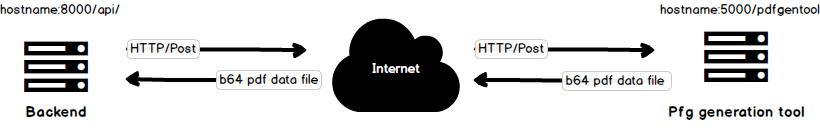
\includegraphics[scale=0.5]{sections/arquitectura/pdfgentool_arch.png}
%\centering
%\caption{Arquitectura generació de documents}
%\label{fig:pdfgentool_arch}
%\end{figure}
%\newline 
Com indica el títol d'aquest TFG, un dels objectius principals és desenvolupar un sistema per a l'emissió (entre altres coses) de consentiments informats.\\
\newline Donada la importància del cas i amb vistes a una possible i futura ampliació del mòdul concret, s'ha desenvolupat un sistema independent per a la generació de documents.\\
%\newline Aquest nou sistema té els casos d'us il·lustrats a la Figura \ref{fig:pdfgentool_usecase}:
%\subsubsection{Casos d'ús}
\begin{figure}[h]
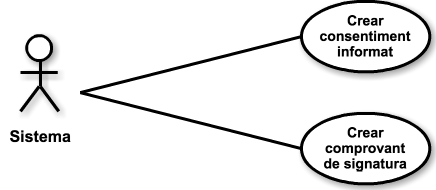
\includegraphics[scale=0.5]{sections/arquitectura/documentGen_usecase.png}
\centering
\caption{Sistema de generació de documents - casos d'ús}
\label{fig:pdfgentool_usecase}
\end{figure}
\newline De la figura anterior (Figura \ref{fig:pdfgentool_usecase}), en podem extreure les diferents funcionalitats que tindrà aquest sistema:
\begin{itemize}
    \item Per una banda, i possiblement la més important, la generació de consentiments informats.\\
    Es considera una de les característiques claus del projecte.\\
    La generació d'aquests documents ha de ser dinàmica, és a dir, donat un \textit{template} bàsic, s'ha d'emplenar de forma adequada amb les dades guardades a la BD i generar-ne el consentiment.
    \item Per altra banda, a mesura que ha avançat el projecte (secció \nameref{desenvolupament} per a més detalls) ha sorgit la necessitat de generar un segon document. Aquest actua com a comprovant de signatura en el procés de petició de servei.\\
    De la mateixa manera que el consentiment informat, aquest document també requereix de contingut dinàmic.
\end{itemize}
Com es diu a l'inici d'aquesta secció, la generació de documents es genera en un mòdul independent al \textit{backend} del projecte.\\
El mòdul de generació de documents està pensat com una API Rest, per tant, la comunicació entre el backend i aquest mòdul es farà via peticions \textit{HTTP/Post}.\\
\newline El \textit{backend} enviarà dades en format JSON\footnote{JavaScript Object Notation} i el sistema de generació donarà com a resposta, en cas de que les dades siguin vàlides, el contingut del document codificat en base64.\\
\newline Com a detall, aquest sistema de generació de documents no té persistència (ni llegeix ni escriu a base de dades), simplement incrusta les dades que rep a cada \textit{request} dins d'una plantilla pre-definida en funció de si s'ha de generar un consentiment o bé un comprovant.

